\documentclass{../../missal-sheet}

\begin{document}

\chapter*{Evangelium Passionis et Mortis domini Secundum Matth\'{\ae}um}

\begin{center}
 Matthew 26, 36-75; 27, 1-60
\end{center}

\begin{rubricbox}
{\color{red} The Gospel procession having taken place, the clerics assemble themselves on the Gospel side, facing liturgical north. The Passion Narrative is chanted, with \textit{four} parts contributing: The Chronicler (symbolized by a letter `C'), Christ (symbolized by a `\maltese'), a singular Synagogue part (symbolized by a `S'), and a plural Synagogue part, known as the `Turba', literally meaning `crowd' (referred to below by the word `Turba').  The Chronicler begins the chanting of the Passion Narrative. For ease of chanting, the singular Synagogue part has been tranposed down a perfect fourth from its original setting.}
\end{rubricbox}

% Page 1:

\gresetinitiallines{1}
\gregorioscore{matthew_passion_1}

% Page 2:

\gresetinitiallines{0}
\gregorioscore{matthew_passion_2}

% Page 3:

\gresetinitiallines{0}
\gregorioscore{matthew_passion_3}

% Page 4:

\gresetinitiallines{0}
\gregorioscore{Victoria/matthew_victoria_passion_4a}

{\color{red}\textit{The Turba sings the following:}}

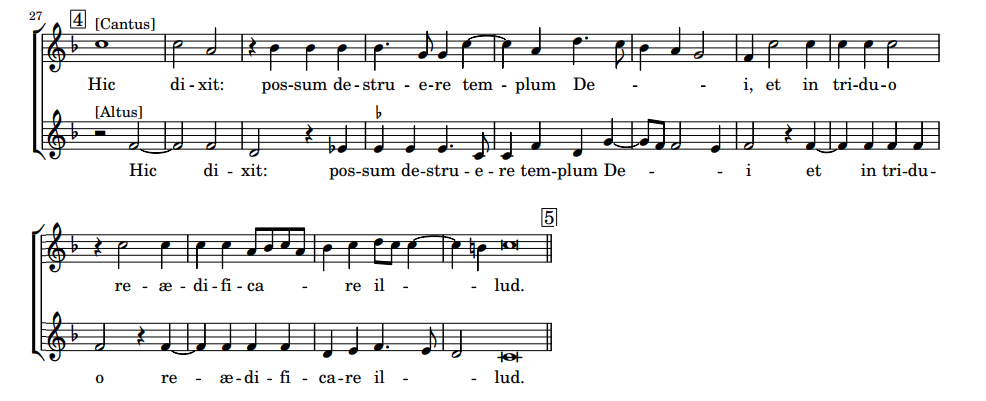
\includegraphics[width=\textwidth]{Victoria/Polyphony/turba1_fixed}

\gresetinitiallines{0}
\gregorioscore{Victoria/matthew_victoria_passion_4b}

% Page 5:

\gresetinitiallines{0}
\gregorioscore{Victoria/matthew_victoria_passion_5a}

{\color{red}\textit{Turba:}}

\begin{center}
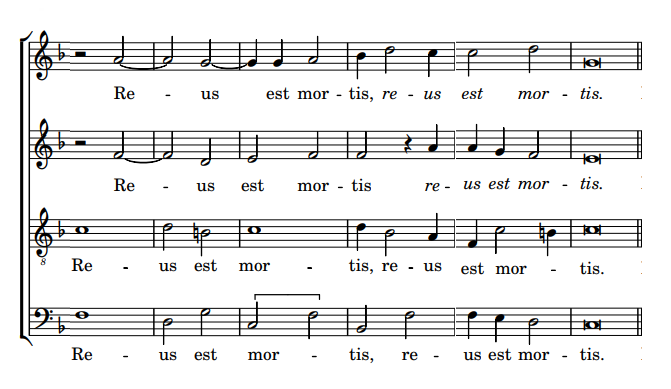
\includegraphics[width=0.75\textwidth]{Victoria/Polyphony/turba2_fixed}
\end{center}

\gresetinitiallines{0}
\gregorioscore{Victoria/matthew_victoria_passion_5b}

{\color{red}\textit{Turba:}}

\begin{center}
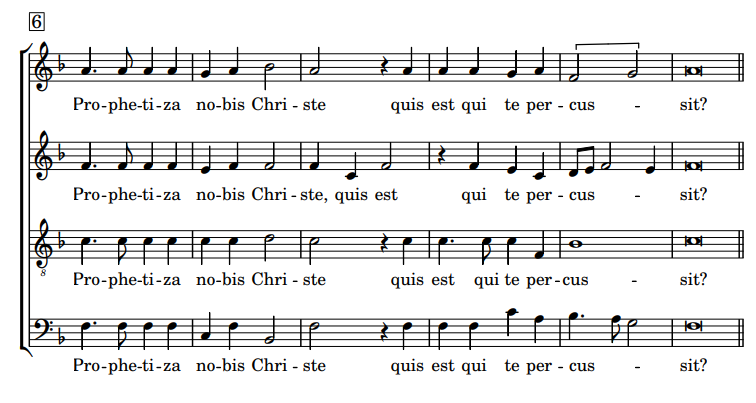
\includegraphics[width=0.85\textwidth]{Victoria/Polyphony/turba3_fixed}
\end{center}

% Page 6:

\gresetinitiallines{0}
\gregorioscore{Victoria/matthew_victoria_passion_6a}

{\color{red}\textit{Turba:}}

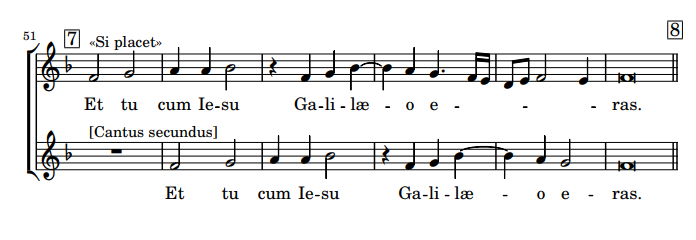
\includegraphics{Victoria/Polyphony/turba4_fixed}

\gresetinitiallines{0}
\gregorioscore{Victoria/matthew_victoria_passion_6b}

{\color{red}\textit{Turba:}}

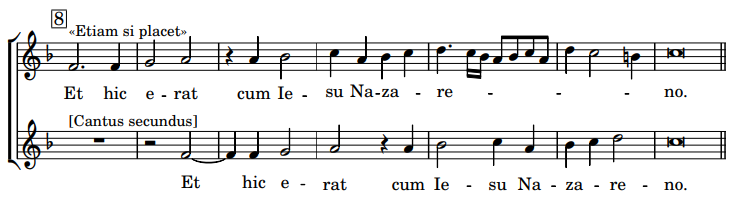
\includegraphics{Victoria/Polyphony/turba5_fixed}

\gresetinitiallines{0}
\gregorioscore{Victoria/matthew_victoria_passion_6c}

%\vfill
\pagebreak

% Page 7:

{\color{red}\textit{Turba:}}

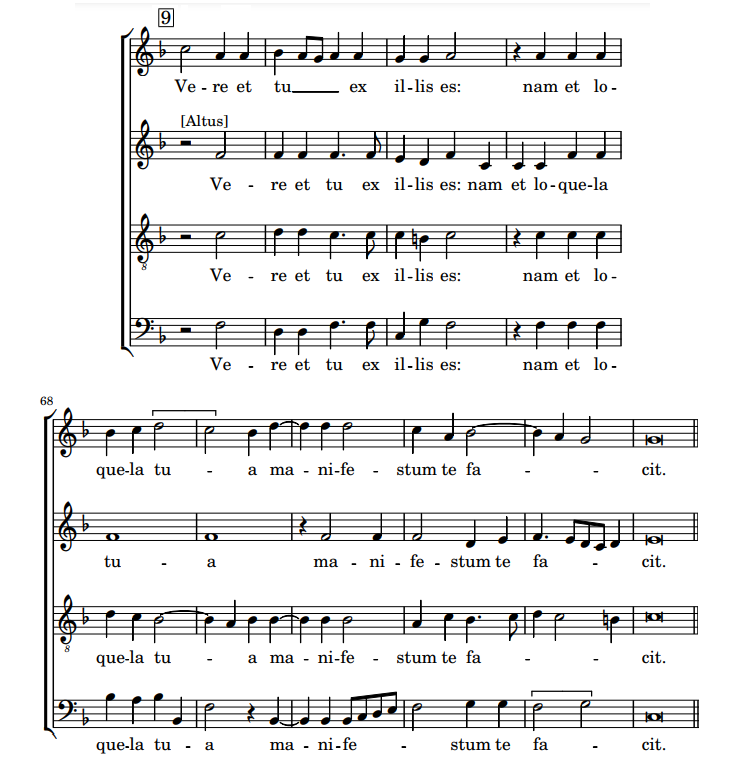
\includegraphics[width=\textwidth]{Victoria/Polyphony/turba6_fixed}

\gresetinitiallines{0}
\gregorioscore{Victoria/matthew_victoria_passion_7}

\vfill\pagebreak

% Page 8:

\gresetinitiallines{0}
\gregorioscore{Victoria/matthew_victoria_passion_8a}

{\color{red}\textit{Turba:}}

\begin{center}
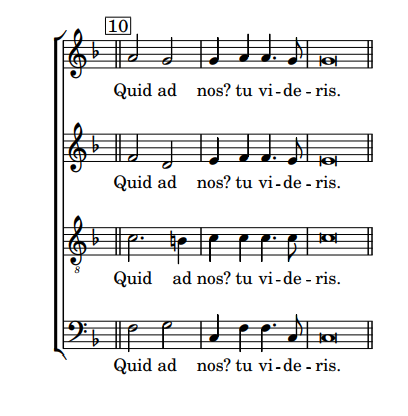
\includegraphics[width=0.5\textwidth]{Victoria/Polyphony/turba7_fixed}
\end{center}

\gresetinitiallines{0}
\gregorioscore{Victoria/matthew_victoria_passion_8b}

%\vfill
\pagebreak

% Page 9:

{\color{red}\textit{Turba:}}

\begin{center}
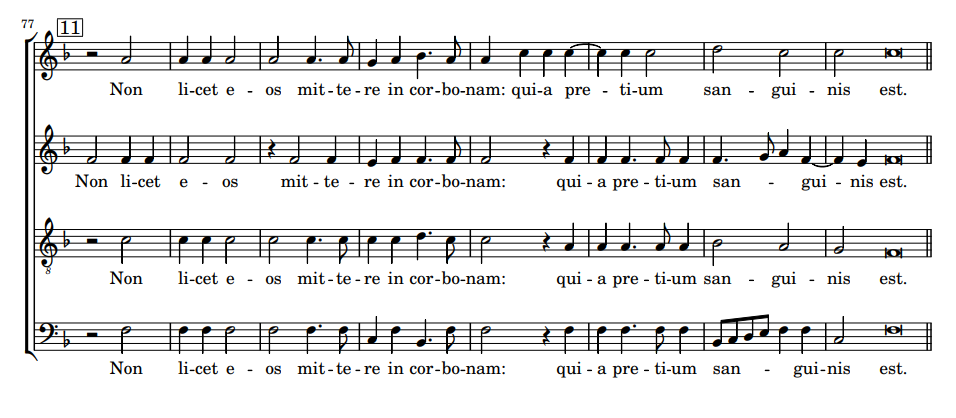
\includegraphics[width=\textwidth]{Victoria/Polyphony/turba8_fixed}
\end{center}

\gresetinitiallines{0}
\gregorioscore{Victoria/matthew_victoria_passion_9}

%\vfill
\pagebreak

% Page 10:

\begin{center}
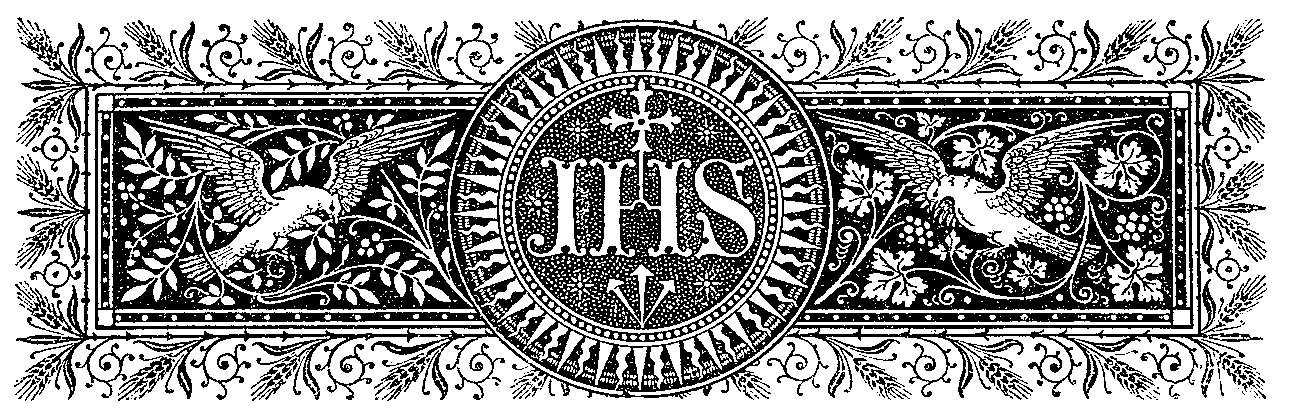
\includegraphics[width=0.8\textwidth]{Victoria/IHS-with-birds-and-flowers}
\end{center}

\gresetinitiallines{0}
\gregorioscore{Victoria/matthew_victoria_passion_10}

%\vfill
\pagebreak

% Page 11:

\gresetinitiallines{0}
\gregorioscore{Victoria/matthew_victoria_passion_11a}

{\color{red}\textit{Turba:}}

\begin{center}
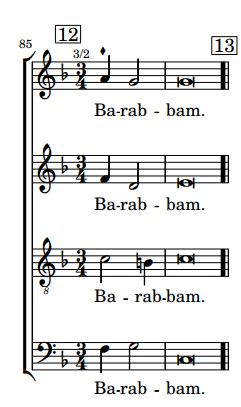
\includegraphics[width=0.3\textwidth]{Victoria/Polyphony/turba9_fixed}
\end{center}

\gresetinitiallines{0}
\gregorioscore{Victoria/matthew_victoria_passion_11b}

{\color{red}\textit{Turba:}}

\begin{center}
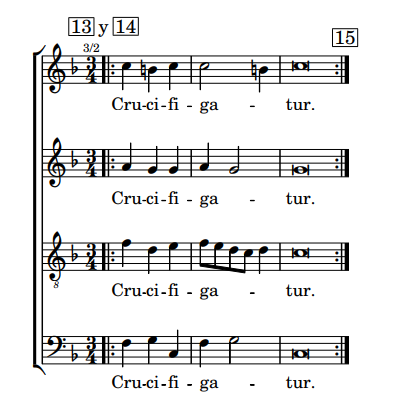
\includegraphics[width=0.45\textwidth]{Victoria/Polyphony/turba10_fixed}
\end{center}

\vfill\pagebreak

% Page 12:

\gresetinitiallines{0}
\gregorioscore{Victoria/matthew_victoria_passion_12a}

{\color{red}\textit{Turba:}}

\begin{center}
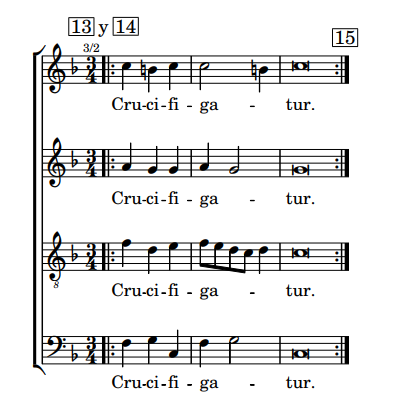
\includegraphics[width=0.4\textwidth]{Victoria/Polyphony/turba11_fixed}
\end{center}

\gresetinitiallines{0}
\gregorioscore{Victoria/matthew_victoria_passion_12b}

{\color{red}\textit{Turba:}}

\begin{center}
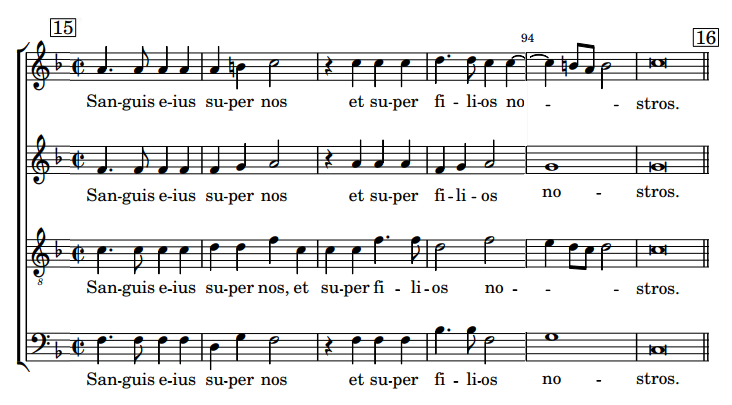
\includegraphics[width=0.75\textwidth]{Victoria/Polyphony/turba12_fixed}
\end{center}

%\vfill
\pagebreak

% Page 13:

\gresetinitiallines{0}
\gregorioscore{Victoria/matthew_victoria_passion_13a}

{\color{red}\textit{Turba:}}

\begin{center}
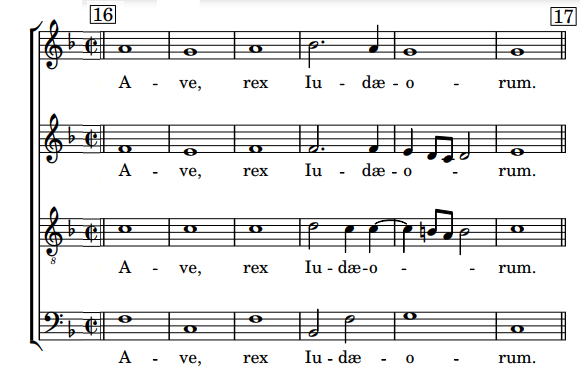
\includegraphics[width=0.8\textwidth]{Victoria/Polyphony/turba13_fixed}
\end{center}

\gresetinitiallines{0}
\gregorioscore{Victoria/matthew_victoria_passion_13b}

\vfill\pagebreak

% Page 14:

\gresetinitiallines{0}
\gregorioscore{Victoria/matthew_victoria_passion_14}

\pagebreak

% Page 15:

{\color{red}\textit{Turba:}}

\begin{center}
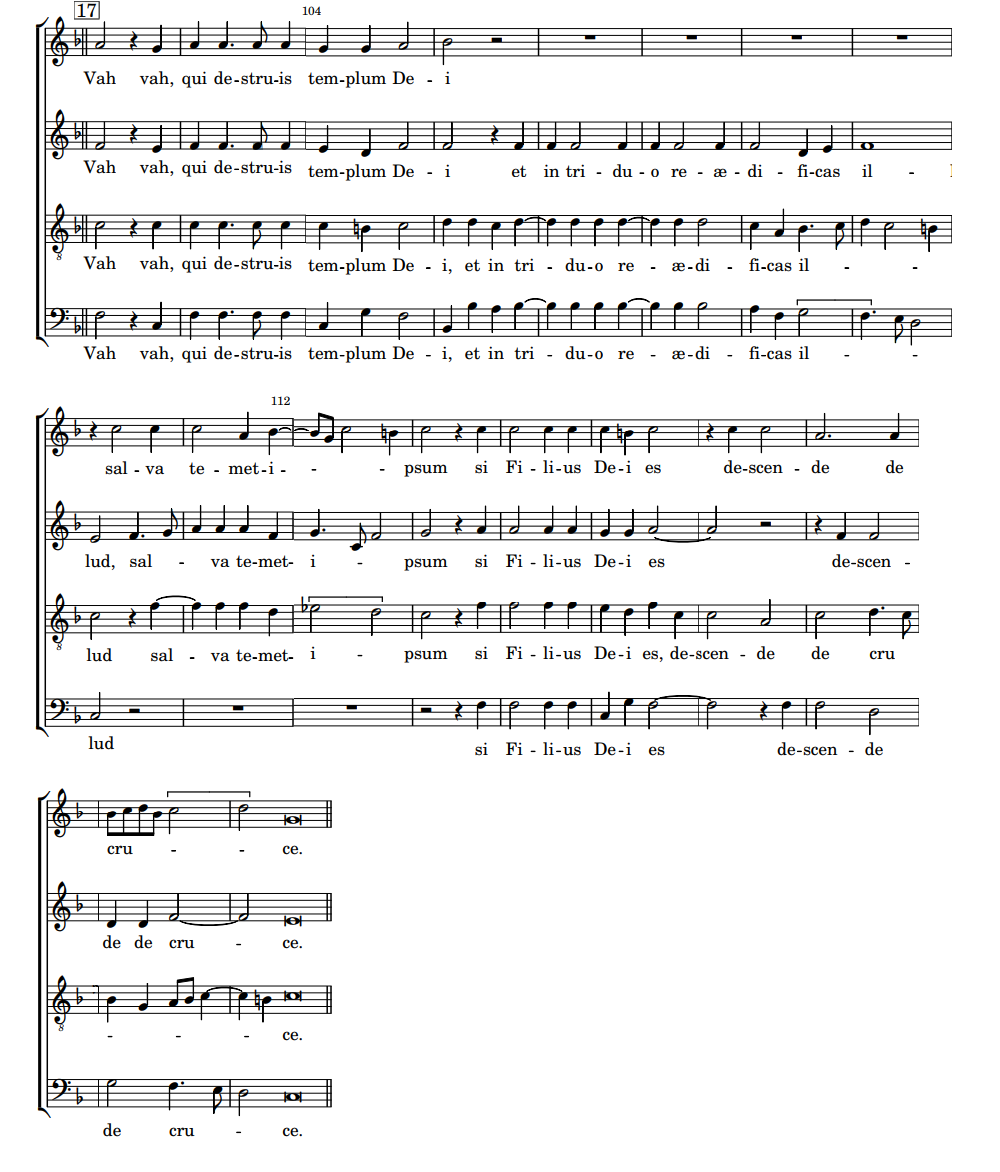
\includegraphics[width=\textwidth]{Victoria/Polyphony/turba14_fixed}
\end{center}

\gresetinitiallines{0}
\gregorioscore{Victoria/matthew_victoria_passion_15}

\vfill\pagebreak

% Page 16:

{\color{red}\textit{Turba:}}

\begin{center}
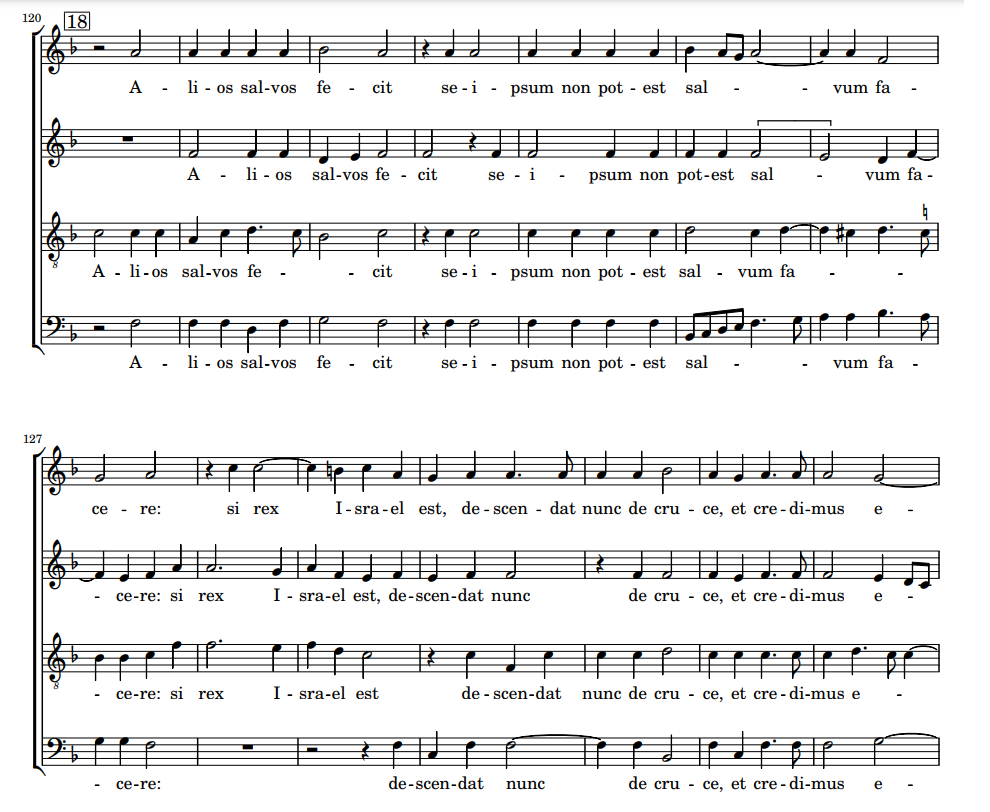
\includegraphics[width=0.85\textwidth]{Victoria/Polyphony/turba15a_fixed}
\end{center}

\begin{center}
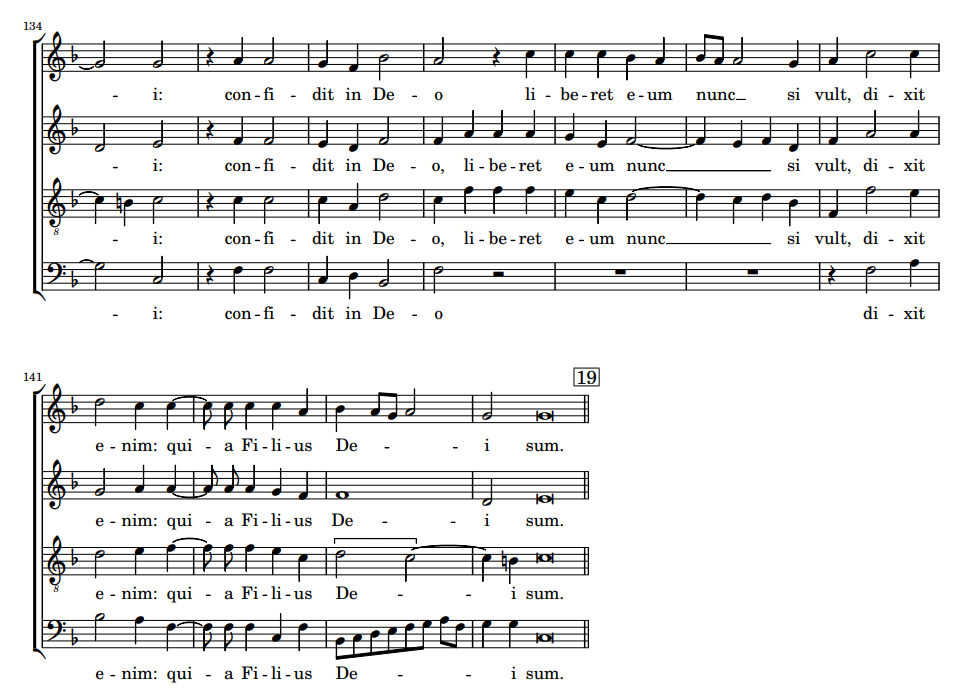
\includegraphics[width=0.85\textwidth]{Victoria/Polyphony/turba15b_fixed}
\end{center}

\vfill\pagebreak

% Page 17:

\gresetinitiallines{0}
\gregorioscore{Victoria/matthew_victoria_passion_16a}

{\color{red}\textit{Turba:}}

\begin{center}
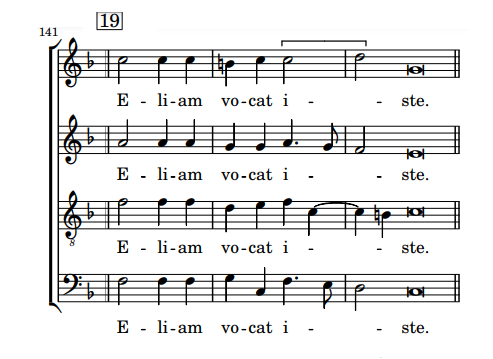
\includegraphics[width=0.7\textwidth]{Victoria/Polyphony/turba16_fixed}
\end{center}

\gresetinitiallines{0}
\gregorioscore{Victoria/matthew_victoria_passion_16b}

\pagebreak

% Page 18:

{\color{red}\textit{Turba:}}

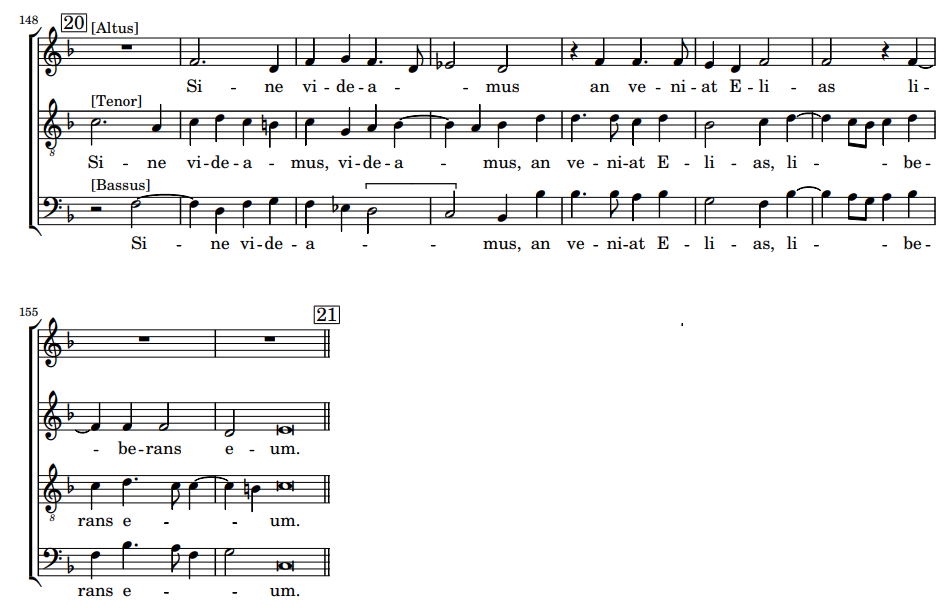
\includegraphics[width=\textwidth]{Victoria/Polyphony/turba17_fixed}

\gresetinitiallines{0}
\gregorioscore{Victoria/matthew_victoria_passion_17}

%\vfill
\pagebreak

% Page 19:

{\color{red}\textit{Turba:}}

\begin{center}
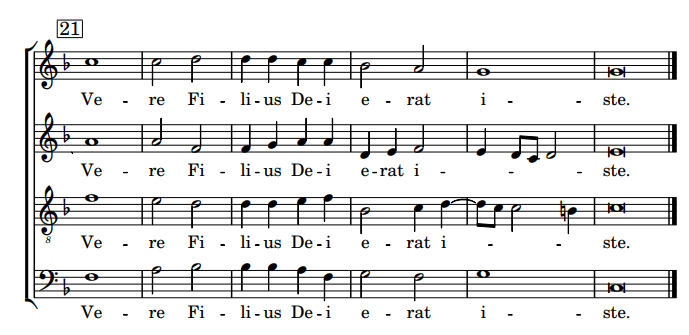
\includegraphics[width=0.9\textwidth]{Victoria/Polyphony/turba18_fixed}
\end{center}

\gresetinitiallines{0}
\gregorioscore{Victoria/matthew_victoria_passion_18}

\end{document}